% Made up for the tikra benchmark.
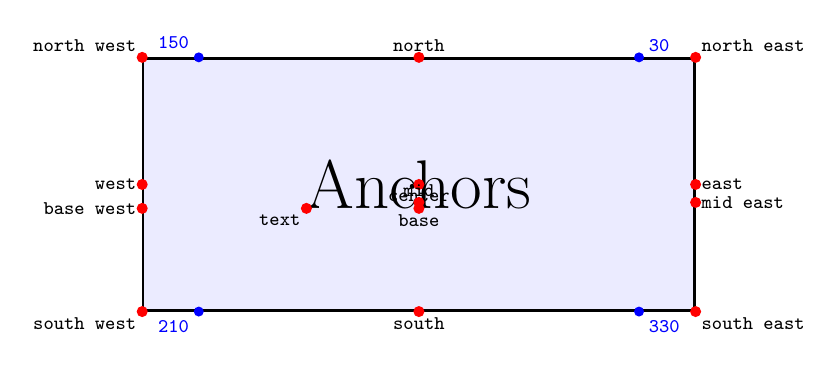
\begin{tikzpicture}
  \node[draw, thick, fill=blue!8, minimum width=7cm, minimum height=3.2cm, font=\Huge] (n) {Anchors};
  \foreach \a/\p in {north/above, south/below, east/right, west/left, north east/above right,
      north west/above left, south east/below right, south west/below left, center/below, text/below left,
      base/below, mid/above, mid east/right, base west/left} {
    \fill[red] (n.\a) circle (2pt);
    \node[\p, font=\scriptsize\ttfamily, inner sep=2pt] at (n.\a) {\a};
  }
  \foreach \ang in {30,150,210,330} {
    \pgfmathtruncatemacro\opp{mod(\ang+180,360)}
    \fill[blue] (n.\ang) circle (1.8pt);
    \node[font=\scriptsize\ttfamily, blue, anchor=\opp] at (n.\ang) {\ang};
  }
\end{tikzpicture}
